\chapter{Array}

Sebuah {\bf array}
adalah sebuah kumpulan nilai di mana setiap nilai tersebut diidentifikasikan dengan sebuah indeks.
Kamu dapat membuat array dengan
{\tt int}, {\tt double}, atau dengan tipe data lainnya, 
tetapi semua nilai di dalam sebuah array harus memiliki tipe data yang sama.

Secara sintaks, tipe data pada array terlihat seperti tipe data pada Java lainnya hanya saja tipe-tipe data tersebut 
diikuti dengan {\tt []}.  Sebagai contoh, {\tt int[]} adalah tipe ``array
integer'' dan {\tt double[]} adalah tipe ``array double.''

Kamu dapat mendeklarasikan variabel dengan tipe ini dengan cara biasa:

\begin{lstlisting}
    int[] count;
    double[] values;
\end{lstlisting}
%
Sebelum anda menginisialisasikan variabel-variabel tersebut, mereka akan diatur menjadi {\tt null}.
Untuk membuat array itu sendiri, gunakan {\tt new}.

\begin{lstlisting}
    count = new int[4];
    values = new double[size];
\end{lstlisting}
%
Perintah pertama membuat {\tt count} merujuk kepada sebuah array dengan 4 integer;
integers; dan perintah kedua membuat {\tt values} merujuk kepada array {\tt
double}s.  Jumlah elemen dalam {\tt values} bergantung kepada {\tt
size}.  Anda dapat menggunakan ekspresi integer lainnya sebagai ukuran dari sebuah array.

\index{null}
\index{state diagram}

Figur di bawah ini menunjukkan bagaimana array direpresentasinya dengan bentuk diagram:


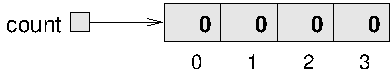
\includegraphics{array.pdf}


Angka dengan ukuran besar yang berada di dalam kotak adalah {\bf elements} dari sebuah array.  Sedangkan angka dengan ukuran kecil yang berada di luar kotak adalah indeks yang digunakan untuk mengidentifikasikan setiap kotak.  Ketika anda menyediakan sebuah array dengan
 {\tt int}, elemen pada array tersebut akan diinisialisasikan ke nol.


\section{Mengakses Elemen}
\index{element}
\index{array!element}

Untuk menyimpan nilai pada array, kita menggunakan operator 
{\tt []}.  Sebagai contoh {\tt count[0]} merujuk pada elemen
``ke-nol'' pada array, dan {\tt count[1]} merujuk pada elemen
``ke-satu''.  Anda dapat menggunakan operator {\tt []} di mana saja dengan ekspresi seperti berikut:

\begin{lstlisting}
    count[0] = 7;
    count[1] = count[0] * 2;
    count[2]++;
    count[3] -= 60;
\end{lstlisting}
%
Semua ekspresi di atas adalah perintah statement yang dibolehkan. Berikut ini adalah hasil dari potongan kode tersebut:


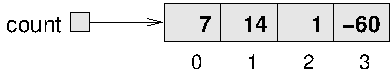
\includegraphics{array2.pdf}


Elemen-elemen pada array tersebut dinomorkan dari 0 ke 3, hal ini berarti bahwa tidak ada elemen dengan indeks 4.  Hal ini tidak terdengar asing, karena kita telah melihat hal yang sama dengan 
indeks pada {\tt String}.  Namun, biasanya eror sangat sering ditemukan ketika kita melewati batas dari sebuah array, yang akan melempar 
{\tt ArrayOutOfBoundsException}.
\index{exception!ArrayOutOfBounds}
\index{run-time error}
\index{index}

Anda dapat menggunakan ekspresi apapun sebagai indeks, selama tipe datanya {\tt
int}. Salah satu cara yang umum digunakan untuk memberi indeks pada array adalah dengan menggunakan variabel perulangan. Sebagai contoh:
\index{expression}

\begin{lstlisting}
    int i = 0;
    while (i < 4) {
        System.out.println(count[i]);
        i++;
    }
\end{lstlisting}
%
Ini merupakan perulangan {\tt while} standar yang menghitung dari 0 sampai 4, dan ketika variabel perulangan {\tt i} adalah 4, pengkondisian akan gagal dan perulangan akan berhenti.  Oleh karena itu, tubuh dari perulangan tersebut hanya dieksekusi ketika {\tt i} bernilai 0, 1, 2 and 3.

\index{loop}
\index{loop variable}
\index{variable!loop}

Setiap saat melewati perulangan kita menggunakan {\tt i} sebagai indeks untuk array, dan mencetak elemen ke-{\tt i}.  Tipe cara pelintasan array ini adalah cara yang umum digunakan.


\section{Menyalin array}
\index{array!copying}

Ketika kamu menyalin sebuah variabel array, perlu diingat bahwa kamu menyalin referensi untuk sebuah array. Sebagai contoh:

\begin{lstlisting}
    double[] a = new double [3];
    double[] b = a;
\end{lstlisting}
%
Kode ini membuat sebuah array dengan tiga {\tt double}, dan
dan mengatur dua variabel berbeda untuk merujuk pada array tersebut.
Situasi ini merupakan bentuk dari aliasing.


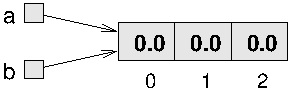
\includegraphics{array3.pdf}


Semua perubahan di salah satu array akan terefleksikan di array satunya. Hal ini bukanlah sifat yang kamu inginkan; seringkali kamu ingin mengalokasikan sebuah array baru dan menyalin elemen-elemen dari satu array ke array lainnya.

\begin{lstlisting}
    double[] b = new double [3];

    int i = 0;
    while (i < 4) {
      b[i] = a[i];
      i++;
    }
\end{lstlisting}


\section{Array dan obyek}
\index{object!compared to array}
\index{array!compared to object}

Dalam banyak hal, array memiliki sifat seperti obyek:

\begin{itemize}

\item Ketika kamu mendeklarasikan sebuah variabel array, kamu akan mendapatkan referensi untuk sebuah array.

\item Kamu harus menggunakan {\tt new} untuk membuat array itu sendiri.

\item Ketika kamu memberikan sebuah array sebagai argumen, kamu memberikan referensi, hal ini berarti bahwa metode yang dipanggil bisa mengubah isi dari sebuah array.

\end{itemize}

Beberapa objek yang pernah kita bahas, seperti {\tt Rectangles}, mirip seperti array dalam arti array dan objek merupakan kumpulan nilai.  Hal ini mengundang pertanyaan, ``Mengapa array dengan 4 integer tadi berbeda dengan objek Rectangle?''
\index{collection}

Bila kamu kembali ke definisi ``array'' pada awal bab ini, kamu akan melihat sebuah perbedaan: elemen dari sebuah array diidentifikasi dengan indeks, dan elemen dari sebuah objek memiliki nama.

Perbedaan lainnya adalah elemen pada array harus memiliki tipe data yang sama. Objek dapat memiliki instansi variabel dengan tipe data yang berbeda.


\section{Perulangan {\tt for}}
\label{for}

Perulangan yang telah kita tuliskan memiliki sejumlah elemen yang sama. Semua perulangan tersebut dimulai dengan menginisialisasikan sebuah variabel; terdapat pengujian pada perulangan tersebut, atau kondisi, yang bergantung pada variabel tersebut; dan di dalam perulangan tersebut dilakukan suatu hal untuk variabel tersebut, contohnya seperti men-increment variabel itu.

\index{loop!for}
\index{for}
\index{statement!for}

Tipe perulangan seperti ini sudah sangat umum digunakan. Ada cara statement perulangan lain, bernama {\tt for}, yang dapat mengekspresikan perulangan
dengan cara yang lebih singkat. Sintaks umumnya adalah seperti berikut:

\begin{lstlisting}
    for (INITIALIZER; CONDITION; INCREMENTOR) {
        BODY
    }
\end{lstlisting}
%
Statement ini ekuivalen dengan

\begin{lstlisting}
    INITIALIZER;
    while (CONDITION) {
        BODY
        INCREMENTOR
    }
\end{lstlisting}
%
dengan perbedaan bahwa perulangan ini lebih ringkas, dan karena perulangan ini memiliki semua statement yang berkaitan dengan sebuah perulangan dalam satu tempat, maka perulangan ini lebih mudah dibaca. Sebagai contoh:

\begin{lstlisting}
    for (int i = 0; i < 4; i++) {
        System.out.println(count[i]);
    }
\end{lstlisting}
%
ekuivalen dengan

\begin{lstlisting}
    int i = 0;
    while (i < 4) {
        System.out.println(count[i]);
        i++;
    }
\end{lstlisting}


\section{Panjang array}
\index{length!array}
\index{array!length}

Semua aray memiliki satu variabel instansi: {\tt length}.
Sesuai dengan namanya, variabel instansi tersebut memuat panjang dari sebuah array  (jumlah elemen). Merupakan cara yang lebih baik untuk menggunakannya sebagai batas atas dari sebuah perulangan, daripada menggunakan nilai konstan.  Dengan cara ini, jika ukuran array berubah, kamu tidak perlu memeriksa seluruh program untuk mengganti seluruh perulangan, perulangan akan bekerja dengan baik untuk berbagai macam ukuran array.

\begin{lstlisting}
    for (int i = 0; i < a.length; i++) {
        b[i] = a[i];
    }
\end{lstlisting}
%
Pada saat terakhir badan perulangan dieksekusi, {\tt i}
bernilai {\tt a.length - 1}, yang merupakan indeks dari elemen terakhir. Ketika
{\tt i} sama dengan {\tt a.length}, kondisi gagal dan badan perulangan tidak akan dieksekusi, yang berarti hal ini adalah hal baik, karena kalau tidak begitu, perulangan tersebut akan melempar eksepsi.  Kode ini memiliki asumsi bahwa array {\tt b} memuat elemen setidaknya sebanyak elemen pada {\tt a}.


\section{Angka acak}
\label{random}
\label{pseudorandom}
\index{random number}
\index{deterministic}
\index{nondeterministic}

Hampir semua program komputer melakukan hal yang sama setiap kali mereka dieksekusi. Sifat ini disebut sebagai {\bf deterministik}.  Biasanya, determinisme adalah  hal yang baik karena kita menginginkan perhitungan yang sama dari program-program yang berbeda untuk mengeluarkan hasil yang sama. Akan tetapi, ada beberapa aplikasi di mana kita menginginkan komputer melakukan hal yang tidak terduga. Permainan merupakan contoh yang kentara, tetapi masih ada juga aplikasi lainnya.

Membuat sebuah program benar-benar {\bf nondeterministik} bukanlah hal yang mudah, akan tetapi ada cara untuk membuatnya setidaknya terlihat nondeterministik. Salah satunya adalah dengan memperoleh angka acak dan menggunakannya untuk menentukan hasil dari sebuah program. Java menyediakan sebuah metode yang menghasilkan angka 
{\bf pseudorandom}, yang mungkin tidak sepenuhnya acak, tetapi mungkin cocok untuk keperluan kita.

Cek dokumentasi metode {\tt random} dalam class {\tt
Math}.  Nilai pengembaliannya adalah sebuah {\tt double} di antara 0.0 dan 1.0.
Untuk lebih jelasnya, lebih besar dari atau sama dengan 0.0 dan kurang dari 1.0.  Setiap kali kamu memanggil {\tt random} kamu akan mendapat angka selanjutnya dalam urutan pseudorandom.
Untuk melihat contohnya, jalankan perulangan berikut:

\begin{lstlisting}
    for (int i = 0; i < 10; i++) {
        double x = Math.random();
        System.out.println(x);
    }
\end{lstlisting}
%
Untuk memperoleh sebuah {\tt double} di antara 0.0 dan sebuah batas atas seperti
{\tt high}, kamu dapat mengalikan {\tt x} dengan {\tt high}.


\section{Array dengan angka acak}
\label{randarray}

Bagaimana cara kamu memperoleh integer acak di antara {\tt low} dan {\tt high}?
Jika implementasi {\tt randomInt} milikmu benar, setiap nilai yang berada di antara {\tt low} sampai {\tt high-1} seharusnya
memiliki peluang yang sama.  Jika kamu menghasilkan sebuah kumpulan angka yang panjang, setiap nilai harus muncul, setidaknya mendekati, dengan jumlah kemunculan yang sama.

Salah satu cara untuk menguji metode kamu adalah dengan menentukan angka dengan jumlah yang banyak dengan nilai acak, simpan nilai tersebut di dalam sebuah array, dan hitung berapa kali kemunculan tiap nilai tersebut.

Metode berikut ini memiliki satu argument, yaitu ukuran array. Ini akan mengalokasikan array integer baru, mengisinya dengan nilai acak dan mengembalikan referensi kepada array yang baru.

\begin{lstlisting}
  public static int[] randomArray(int n) {
      int[] a = new int[n];
      for (int i = 0; i<a.length; i++) {
          a[i] = randomInt(0, 100);
      }
      return a;
  }
\end{lstlisting}
%
Tipe data pada pengembalian adalah {\tt int[]}, hal ini berarti bahwa metode ini mengembalikan array bertipe integer.
Untuk menguji metode ini, akan lebih mudah kita untuk memiliki metode untuk mencetak isi dari array.

\begin{lstlisting}
  public static void printArray(int[] a) {
      for (int i = 0; i<a.length; i++) {
          System.out.println(a[i]);
      }
  }
\end{lstlisting}
%
Kode berikut menghasilkan sebuah array dan mencetak isinya:

\begin{lstlisting}
    int numValues = 8;
    int[] array = randomArray(numValues);
    printArray(array);
\end{lstlisting}
%
Output yang diperoleh pada mesinku adalah

\begin{verbatim}
27
6
54
62
54
2
44
81
\end{verbatim}
%
Output ini terlihat acak. Hasil yang kamu peroleh mungkin berbeda.

Jika output tersebut adalah nilai ujian (dan nilai-nilai tersebut akan menjadi nilai ujian yang buruk), guru yang menilainya mungkin akan menampilkan hasilnya pada kelasnya dalam bentuk {\bf histogram}, yaitu kumpulan penghitung yang menyimpan jumlah berapa kali sebuah nilai muncul.

\index{histogram}

Dalam nilai ujian, kita mungkin memiliki 10 prnghitung untuk mengetahui berapa banyak siswa yang mendapatkan nilai 90-an, 80-an, dan lain-lain. Pada bagian selanjutnya kita akan mendalami kode untuk membuat sebuah histogram.


\section{Perhitungan}
\index{traverse!array}
\index{array!traverse}
\index{looping and counting}
\index{counter}

Sebuah pendekatan yang baik dalam permasalahan seperti ini adalah dengan membuat metode sederhana yang mudah untuk ditulis, dan mengombinasikannya menjadi sebuah solusi.
Proses seperti itu disebut sebagai {\bf bottom-up development}.
Lihat \ref{http://en.wikipedia.org/wiki/Top-down_and_bottom-up_design}.
\index{program development}

Tidak selalu mudah untuk menentukan di mana kita harus mulai, tetapi salah satu pendekatan terbaik adalah dengan melihat submasalah yang cocok dengan pola yang telah kamu lihat sebelumnya.

Pada bagian~\ref{loopcount}kita telah melihat sebuah perulangan yang melewati setiap huruf dalam sebuah string dan menghitung berapa kali sebuah huruf muncul. Kamu dapat berpikir program ini seperti sebuah contoh dari pola yang dapat dinamakan ``lintasi dan hitung.''  Elemen dari pola ini adalah:

\begin{itemize}

\item Sebuah kumpulan atau penampung yang dapat dilintasi, seperti array atau string.

\item Sebuah penguji yang dapat diaplikasaikan kepada setiap elemen di dalam penampung.

\item Sebuah penghitung yang menyimpan jumlah berapa kali sebuah elemen lulus dalam pengujian.

\end{itemize}

Dalam kasus ini, penampung yang dipakai adalah sebuah array integer. Uji yang dipakai adalah uji apakah sebuah nilai cocok atau tidak pada daerah nilai yang diberikan.

Berikut ini adalah metode yang bernama {\tt inRange} yang menghitung jumlah elemen yang berada di dalam array. Parameternya adalah sebuah array dan dua integer yang menspesifikkan batas bawah dan batas atas sebuah daerah.

\begin{lstlisting}
public static int inRange(int[] a, int low, int high) {
    int count = 0;
    for (int i = 0; i < a.length; i++) {
        if (a[i] >= low && a[i] < high) count++;
    }
    return count;
}
\end{lstlisting}
%
Saya tidak spesifik menuliskan apakah nilai yang sama dengan {\tt low} atau {\tt high} high akan gagal dalam daerah itu, tapi kamu dapat melihat dari kode tersebut bahwa {\tt low} merupakan awal dan {\tt high} merupakan akhir.
Hal tersebut membuat kita tidak menghitung elemen yang sama dua kali.

Sekarang kita dapat mengitung jumlah nilai di dalam daerah yang kita inginkan:

\begin{lstlisting}
int[] scores = randomArray(30);
int a = inRange(scores, 90, 100);
int b = inRange(scores, 80, 90);
int c = inRange(scores, 70, 80);
int d = inRange(scores, 60, 70);
int f = inRange(scores, 0, 60);
\end{lstlisting}


\section{Histogram}
\index{range}
\index{histogram}

Kode ini dijalankan berulang-ulang, dan hal ini masih dapat diterima selama banyaknya daerah yang ingin dihitung kecil. Tetapi bayangkan jika kita ingin menyimpan jumlah berapa kali tiap nilai muncul dengan 100 kemungkinan nilai. Apakah kamu ingin menuliskan ini?

\begin{lstlisting}
int count0 = inRange(scores, 0, 1);
int count1 = inRange(scores, 1, 2);
int count2 = inRange(scores, 2, 3);
...
int count3 = inRange(scores, 99, 100);
\end{lstlisting}

Saya rasa tidak. Apa yang kita inginkan adalah cara untuk menyimpan 100 integer, akan lebih baik jika kita dapat menggunakan indeks untuk mengakses tiap integer. Petunjuk: array.

Pola perhitungan akan tetap sama, baik dengan menggunakan satu penghitung ataupun dengan array berisikan penghitung. Dalam kasus ini, kita menginisialisasikan array di luar perulangan; kemudian, di dalam perulangan, kita memanggil {\tt inRange} dan menyimpan hasilnya:

\begin{lstlisting}
    int[] counts = new int[100];

    for (int i = 0; i < counts.length; i++) {
        counts[i] = inRange(scores, i, i+1);
    }
\end{lstlisting}
%
Satu-satunya hal yang dapat membingungkan di sini adalah kita menggunakan variabel perulangan dalam dua peran: sebagai indeks pada array dan sebagai parameter pada
{\tt inRange}.


\section{Solusi sekali jalan}
\label{singlepass}

Kode-kode di atas bekerja, tetapi tidak begitu efisien. Setiap kali program memanggil metode {\tt inRange}, metode tersebut bekerja melintasi seluruh bagian array.  Setiap jumlah daerah yang dihitung bertambah, setiap itu juga pelintasan bertambah banyak.

Akan lebih baik jika kita membuat hanya satu pengujian pada array, dan untuk setiap nilai, akan dihitung pada daerah mana terdapat nilai tersebut. Kemudian kita men-increment penghitung. Pada contoh ini, komputasi yang dilakukan bersifat trivial, karena kita dapat menggunakan nilai itu sendiri sebagai indeks untuk menjadi array penghitung.

Kode berikut melintasi array skor sekali lalu membuat sebuah histogram.

\begin{lstlisting}
    int[] counts = new int[100];

    for (int i = 0; i < scores.length; i++) {
        int index = scores[i];
        counts[index]++;
    }
\end{lstlisting}


\section{Glosarium}

\begin{description}

\item[array:]  Kumpulan nilai-nilai di mana semua nilai tersebut memiliki tipe data yang sama, dan setiap nilai diidentifikasikan dengan sebuah indeks.

\item[elemen:]  Salah satu nilai yang terdapat pada sebuah array. Operator {\tt []} dipakai untuk memilih sebuah elemen.

\item[indeks:]  Sebuah variabel integer atau nilai yang digunakan untuk mengidentifikasi sebuah elemen pada sebuah array.

\item[deterministik:]  Sebuah program yang akan melakukan hal yang sama setiap kali program tersebut dijalankan.

\item[pseudorandom:]  Sebuah urutan bilangan yang muncul secara acak, tetapi merupakan hasil dari komputasi deterministik.

\item[histogram:]  Sebuah array integer di mana setiap integer menghitung berapa banyak nilai yang berada di dalam sebuah daerah.

\index{array}
\index{element}
\index{index}
\index{deterministic}
\index{pseudorandom}

\end{description}


\section{Latihan}




\subsection{Latihan 12.1}
Tuliskan sebuah metode bernama {\tt cloneArray} yang menggunakan sebuah array integer sebagai parameter, kemudian membuat array yang baru yang memiliki ukuran yang sama dengan array integer tersebut, lalu menyalin elemen dari array pertama ke array kedua dan kemudian akan mengembalikan sebuah referensi untuk array yang baru.



\subsection{Latihan 12.2}
Tuliskan sebuah metode {\tt randomDouble} yang menggunakan dua double, yaitu
{\tt low} dan {\tt high}, dan mengembalikan sebuah double $x$
sehingga $low \le x < high$.



\subsection{Latihan 12.3}
Tuliskan sebuah metode bernama {\tt randomInt} menggunakan dua argumen, yaitu
{\tt low} dan {\tt high}, dan mengemblikan sebuah integer acak di antara
{\tt low} dan {\tt high}, tetapi tidak termasuk {\tt high}.



\subsection{Latihan 12.4}
Rangkumlah kode pada bagian~\ref{singlepass} pada sebuah metod bernama
{\tt makeHist} yang menggunakan array berisi skor dan mengembalikan histogram nilai di dalam array.



\subsection{Latihan 12.5}
Tuliskan sebuah metode bernama {\tt areFactors} yang menggunakan sebuah integer {\tt n} dan sebuah array bertipe integer, dan mengembalikan
{\tt true} jika semua bilangan di dalam array tersebut adalah faktor dari {\tt n}
({\tt n} dapat dibagi oleh semua bilangan tersebut).
PETUNJUK: Lihat Latihan \textbf{6.1}.


\subsection{Latihan 12.6}
Tuliskan sebuah metode yang menggunakan sebuah array bertipe integer dan sebuah integer bernama
{\tt target} sebagai argumen, dan mengembalikan indeks pertama di mana
{\tt target} muncul di dalam array jika hal tersebut terjadi. Jika tidak, maka metode akan mengembalikan -1.


\subsection{Latihan 12.7}
Ada beberapa programmer yang tidak setuju dengan peraturan umum yang menyebutkan bahwa variabel dan metode harus diberi nama yang berarti. Akan tetapi, mereka berpikir bahwa variabel dan metode harus dinamai dengan nama buah.

Untuk setiap metode berikut, tuliskan satu kalimat yang mendeskripsikan secara abstrak apa yang metode tersebut lakukan. Untuk setiap variabel, identifikasikan peran-peran dari variabel tersebut.

\begin{lstlisting}
public static int banana(int[] a) {
    int grape = 0;
    int i = 0;
    while (i < a.length) {
        grape = grape + a[i];
        i++;
    }
    return grape;
}

public static int apple(int[] a, int p) {
    int i = 0;
    int pear = 0;
    while (i < a.length) {
        if (a[i] == p) pear++;
        i++;
    }
    return pear;
}

public static int grapefruit(int[] a, int p) {
    for (int i = 0; i<a.length; i++) {
        if (a[i] == p) return i;
    }
    return -1;
}
\end{lstlisting}
Tujuan dari latihan ini adalah untuk latihan membaca kode dan mengetahui pola komputasi yang pernah kita bahas.



\subsection{Latihan 12.8}
\begin{enumerate}

\item Apakah output dari program berikut?

\item Gambarkan diagram stack yang menunjukkan keadaan program sesaat sebelum {\tt mus} mengembalikan nilai.

\item Jelaskan dengan singkat apa yang metode {\tt mus} lakukan.
\end{enumerate}

\begin{lstlisting}
public static int[] make(int n) {
    int[] a = new int[n];

    for (int i = 0; i < n; i++) {
        a[i] = i+1;
    }
    return a;
}

public static void dub(int[] jub) {
    for (int i = 0; i < jub.length; i++) {
        jub[i] *= 2;
    }
}

public static int mus(int[] zoo) {
    int fus = 0;
    for (int i = 0; i < zoo.length; i++) {
        fus = fus + zoo[i];
    }
    return fus;
}

public static void main(String[] args) {
    int[] bob = make(5);
    dub(bob);

    System.out.println(mus(bob));
}
\end{lstlisting}



\subsection{Latihan 12.9}
Kebanyakan pola yang telah kita bahas untuk melintasi array dapat dituliskan secara rekursif. Memang tidak umum untuk melakukan hal tersebut, tetapi latihan berikut adalah latihan yang akan berguna ke depannya.

\begin{enumerate}

\item Tuliskan sebuah metode bernama {\tt maxInRange} yang menggunakan sebuah array bertipe integer dan sebuah daerah indeks ({\tt lowIndex} dan {\tt highIndex}), dan mencari nilai maksimum dalam array tersebut, yang hanya berada di antara {\tt lowIndex} dan {\tt highIndex}, termasuk kedua batas tersebut.

Metode ini seharusnya merupakan metode rekursif. Jika besar daerah tersebut 1, yang berarti, jika {\tt lowIndex == highIndex}, kita langsung tahu bahwa elemen yang berada di dalam daerah tersebut adalah nilai maksimum. Ini merupakan kasus dasar.

Jika ada lebih dari satu elemen di dalam range, kita dapat memecah array menjadi dua bagian, cari nilai maksimum di setiap bagian, dan cari nilai maksimum dari antara nilai-nilai maksimum yang diperoleh.

\item Metode seperti {\tt maxInRange} mungkin agak aneh untuk digunakan.  Untuk mencari nilai terbesar di dalam sebuah array, kita harus menyediakan daerah yang terdapat seluruh bagian array di dalamnya.

\begin{lstlisting}
    double max = maxInRange(array, 0, a.length-1);
\end{lstlisting}

Tuliskan sebuah metode bernama {\tt max} yang menggunakan sebuah array sebagai parameter dan menggunakan {\tt maxInRange} untuk mencari dan mengembalikan nilai terbesar.
Metode seperti {\tt max} terkadang disebut {\bf metode pembungkus}
karena mereka menyediakan lapisan abstraksi pada metode yang aneh dan membuatnya lebih mudah digunakan.  Metode yang sebenarnya melakukan komputasi disebut {\bf metode pembantu}.

\item Tuliskan sebuah metode dengan versi rekursif dari {\tt find} dengan menggunakan pola pembungkus-pembantu.  {\tt find} menggunakan sebuah array integer dan sebuah integer target.  Metode ini mengembalikan indeks dari tempat pertama integer target muncul di dalam array, atau -1 jika tidak ada.

\end{enumerate}


\subsection{Latihan 12.10}
Salah satu cara yang agak efisien untuk mengurutkan elemen-elemen dalam sebuah array adalah dengan mencari nilai terbesar dan menukarnya dengan elemen pertama, lalu cari nilai terbesar kedua dan menukarnya dengan elemen kedua, dan seterusnya.  Metode ini dinamakan {\bf selection
sort} (lihat \ref{http://en.wikipedia.org/wiki/Selection_sort} ).

\begin{enumerate}

\item Tuliskan sebuah metode bernama {\tt indexOfMaxInRange} yang menggunakan sebuah array bertipe integer, mencari nilai terbesar pada daerah yang diberikan, dan mengembalikan {\em indeks} nilai tersebut.
Kamu dapat memodifikasi versi rekursif dari {\tt maxInRange} atau kamu dapat menulis versi iteratif dari kode awal.

\item Tuliskan sebuah metode bernama {\tt swapElement} yang menggunakan sebuah array bertipe integer dan dua indeks, dan menukar elemen pada indeks-indeks yang diberikan.

\item Tuliskan sebuah metode bernama {\tt selectionSort} yang menggunakan sebuah array bertipe integer dan menggunakan {\tt indexOfMaxInRange} dan {\tt swapElement}
untuk mengurutkan array dari yang terkecil ke terbesar.

\end{enumerate}



\subsection{Latihan 12.11}
Tuliskan sebuah metode bernama {\tt letterHist} yang menggunakan sebuah String sebagai parameter dan mengembalikan sebuah histogram dari huruf-huruf dalam String tersebut.
Elemen ke-nol dari histogram tersebut berisi jumlah huruf a yang berada di dalam String tersebut (huruf besar maupun huruf kecil); elmen ke-25 berisi jumlah huruf z yang berada pada String tersebut. Solusi yang kamu buat hanya memperbolehkan pelintasan String sebanyak satu kali.



\subsection{Latihan 12.12}
Sebuah kata dikatakan “doubloon” jika setiap huruf pada kata tersebut muncul dua kali. Sebagai contoh, berikut ini adalah semua doubloon yang saya temukan di kamusku.

\begin{quote}
Abba, Anna, appall, appearer, appeases, arraigning, beriberi,
bilabial, boob, Caucasus, coco, Dada, deed, Emmett, Hannah,
horseshoer, intestines, Isis, mama, Mimi, murmur, noon, Otto, papa,
peep, reappear, redder, sees, Shanghaiings, Toto
\end{quote}

Tuliskan sebuah metode bernama {\tt isDoubloon} yang mengembalikan {\tt true}
jika kata yang diberikan adalah doubloon dan {\tt false} untuk sebaliknya.



\subsection{Latihan 12.13}
Dua buah kata adalah anagram jika kedua kata tersebut mengandung huruf yang sama (dan jumlah huruf yang sama).  Sebagai contoh, ``stop'' adalah anagram dari ``pots'' dan ``allen downey'' adalah anagram dari ``well annoyed.''

Tuliskan sebuah metode yang menggunakan dua String dan mengembalikan {\tt true} jika kedua String tersebut merupakan anagram dari satu sama lain.

Tantangan opsional: baca huruf-huruf pada kedua String tersebut hanya sekali.



\subsection{Latihan 12.14}
Pada permainan Scrabble, setiap pemain memiliki kumpulan ubin dengan huruf di permukaannya, dan tujuan permainan ini adalah untuk menggunakan huruf-huruf terrsebut untuk mengeja kata. Sistem penilaian pada permainan tersebut cukup rumit, tetapi yang pasti, kata yang lebih panjang akan bernilai lebih banyak daripada kata yang lebih pendek.

Bayangkan kamu diberikan sebuah kumpulan ubin sebagai String, seperti {\tt
"quijibo"} dan kamu diberikan String lain untuk diuji, seperti {\tt "jib"}.
Tuliskan sebuah metode bernama {\tt canSpell} yang menggunakan dua String dan
mengembalikan {\tt true} jika kumpulan ubin tersebut dapat digunakan untuk mengeja sebuah kata.  Kamu mungkin memiliki lebih dari satu ubin dengan huruf yang sama, tetapi kamu boleh menggunakan setiap ubin hanya sekali saja.

Tantangan opsional: baca huruf-huruf pada kedua String tersebut hanya sekali.



\subsection{Latihan 12.15}
Pada permainan Scrabble yang nyata, ada beberapa ubin kosong yang dapat digunakan sebagai wild card; yaitu ubin kosong yang dapat digunakan untuk merepresentasikan huruf apapun.

Pikirkan sebuah algoritma untuk {\tt canSpell} yang dapat berurusan dengan wild
card.  Jangan terganggu dengan detail implementasi seperti bagaimana cara merepresentasikan wild card.  Deskripsikan saja algoritmanya, dengan menggunakan bahasa Inggris, Indonesia, pseudocode, atau Java.




